%% LyX 2.1.4 created this file.  For more info, see http://www.lyx.org/.
%% Do not edit unless you really know what you are doing.
\documentclass[a4paper,twoside,british,cleardoublepage=empty,BCOR15mm,DIV12]{scrreprt}
\usepackage{amsmath}
\usepackage{tgtermes}
\usepackage{tgheros}
\usepackage{tgcursor}
\usepackage{newtxmath}
\usepackage[T1]{fontenc}
\usepackage[utf8]{inputenc}
\usepackage{babel}
\usepackage{float}
\usepackage{graphicx}
\usepackage[unicode=true,pdfusetitle,
 bookmarks=true,bookmarksnumbered=false,bookmarksopen=false,
 breaklinks=false,pdfborder={0 0 1},backref=false,colorlinks=false]
 {hyperref}

\makeatletter

%%%%%%%%%%%%%%%%%%%%%%%%%%%%%% LyX specific LaTeX commands.
\pdfpageheight\paperheight
\pdfpagewidth\paperwidth

\newcommand{\noun}[1]{\textsc{#1}}
%% Because html converters don't know tabularnewline
\providecommand{\tabularnewline}{\\}
\floatstyle{ruled}
\newfloat{algorithm}{tbp}{loa}[chapter]
\providecommand{\algorithmname}{Algorithm}
\floatname{algorithm}{\protect\algorithmname}

%%%%%%%%%%%%%%%%%%%%%%%%%%%%%% User specified LaTeX commands.
%<-------------------------------společná nastavení------------------------------>
\usepackage[numbers,sort&compress]{natbib} %balíček pro citace literatury  
\usepackage{algorithmic}
\usepackage{color}%kvůli barvám ČVUT
\newcommand{\BibTeX}{{\sc Bib}\TeX}%BibTeX logo
\usepackage{multicol}
\usepackage[overload]{textcase}



%<-----------------------------volání stylů----------------------------------------->
% (znak % je označení komentáře: co je za ním, není aktivní)

%<--------matematické písmo--------------------------------------->

%\usepackage[helvet]{packages/sfmath}%matematika ala helvetica



%<------------------------------záhlaví stránek------------------------------------>
%\usepackage{packages/bc-headings}
\usepackage{packages/bc-fancyhdr}

%<------------------------------hlavičky kapitol------------------------------------>
%\usepackage{packages/bc-neueskapitel}
\usepackage{packages/bc-fancychap}

\makeatother

\begin{document}
~\thispagestyle{empty}\begin{center}\pagenumbering{arabic}\vspace{10mm}


\textsf{\textsc{\noun{\LARGE{}Czech Technical University in Prague}}}\\
\vspace{0.5em}
\textsf{\textsc{\noun{\LARGE{}Faculty of Electrical Engineering}}}\\
\vspace*{1em}
\textsf{\textsc{\noun{\Large{}Department of Cybernetics}}}\vspace{15mm}


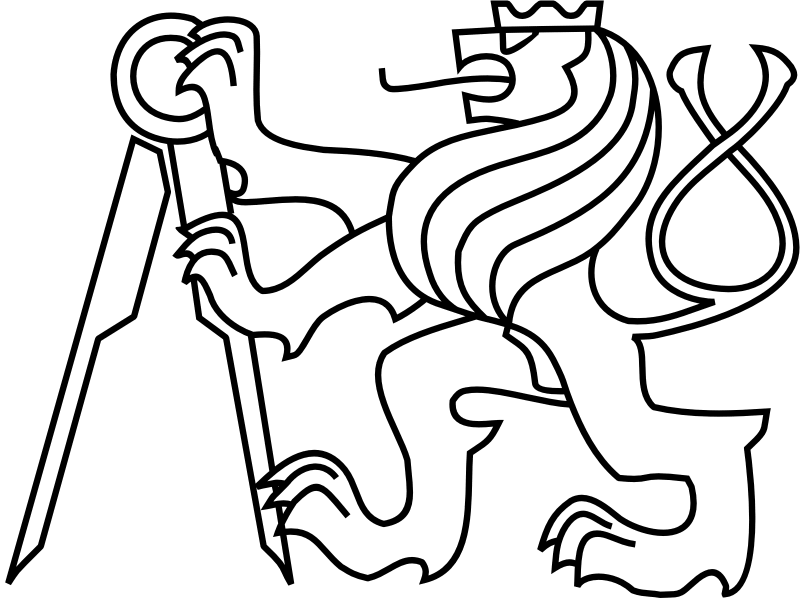
\includegraphics[width=0.3\textwidth]{obrazky/lev}\vspace{15mm}


\textsf{\huge{}BACHELOR THESIS}{\huge \par}

\vspace{15mm}


\textsf{\LARGE{}RRT-path method used for cooperative surveillance
by group of helicopters}{\LARGE \par}

\vspace{10mm}


\end{center} 

\vspace*{\fill}


\vspace{10mm}

\begin{description}
\item [{{\large{}Author:}}] \noindent \textsf{\large{}Matěj Račinský}{\large \par}
\item [{{\large{}Thesis~supervisor:}}] \noindent \textsf{\large{}Dr. Martin
Saska}{\large{}\hfill{}}\textsf{\large{}In Prague,}{\large{} \the\year % nebo doplňte rok vzniku vaší bakalářské práce
}{\large \par}
\end{description}
\clearpage{}

{\small{}\thispagestyle{plain}\addcontentsline{toc}{chapter}{Abstrakt} }{\small \par}

\noindent {\small{}~\vfill{}
}{\small \par}
\begin{description}
\item [{{\small{}Název~práce:}}] \noindent {\small{}Aplikace algoritmu
RRT-path v úloze autonomního dohledu skupinou helikoptér}{\small \par}
\item [{{\small{}Autor:}}] \noindent {\small{}Matěj Račinský}{\small \par}
\item [{{\small{}Katedra~(ústav):}}] \noindent Kate{\small{}dra kybernetiky}{\small \par}
\item [{{\small{}Vedoucí~bakalářské~práce:}}] \noindent Dr. Martin Saska
\item [{{\small{}e-mail~vedoucího:}}] \noindent {\small{}saska@labe.felk.cvut.cz}\\
{\small \par}
\item [{{\small{}Abstrakt}}] \noindent {\small{}V předložené práci studujeme...
Uvede se abstrakt v rozsahu 80 až 200 slov. Lorem ipsum dolor sit
amet, consectetuer adipiscing elit. Ut sit amet sem. Mauris nec turpis
ac sem mollis pretium. Suspendisse neque massa, suscipit id, dictum
in, porta at, quam. Nunc suscipit, pede vel elementum pretium, nisl
urna sodales velit, sit amet auctor elit quam id tellus. Nullam sollicitudin.}{\small \par}
\item [{{\small{}Klíčová~slova:}}] \noindent {\small{}klíčová slova (3
až 5)}\\
{\small \par}
\item [{\rule[0.5ex]{1\linewidth}{1pt}}]~{\small \par}
\item [{{\small{}Title:}}] \noindent {\small{}RRT-path method used for
cooperative surveillance by group of helicopters}{\small \par}
\item [{{\small{}Author:}}] \noindent {\small{}Matěj Račinský}{\small \par}
\item [{{\small{}Department:}}] \noindent {\small{}Department of Cybernetics}{\small \par}
\item [{{\small{}Supervisor:}}] \noindent Dr. Martin Saska
\item [{{\small{}Supervisor's~e-mail~address:}}] \noindent {\small{}saska@labe.felk.cvut.cz}\\
{\small \par}
\item [{{\small{}Abstract}}] \noindent {\small{}In the present work we
study ... Uvede se anglický abstrakt v rozsahu 80 až 200 slov. Lorem
ipsum dolor sit amet, consectetuer adipiscing elit. Ut sit amet sem.
Mauris nec turpis ac sem mollis pretium. Suspendisse neque massa,
suscipit id, dictum in, porta at, quam. Nunc suscipit, pede vel elementum
pretium, nisl urna sodales velit, sit amet auctor elit quam id tellus.
Nullam sollicitudin. Donec hendrerit. Aliquam ac nibh. Vivamus mi.
Sed felis. Proin pretium elit in neque. Pellentesque at turpis. Maecenas
convallis. Vestibulum id lectus. }{\small \par}
\item [{{\small{}Keywords:}}] \noindent {\small{}klíčová slova (3 až 5)
v angličtině}{\small \par}
\end{description}
\cleardoublepage{}\thispagestyle{empty}~{\small{}\addcontentsline{toc}{chapter}{Zadání
práce} }{\small \par}

\thispagestyle{plain}

{\small{}%\setcounter{page}{3} % nastavení číslování stránek
\ }{\small \par}

\noindent {\small{}\vfill{}
 % nastavuje dynamické umístění následujícího textu do spodní části stránky
~}{\small \par}

\noindent {\small{}Prohlašuji, že jsem svou bakalářskou práci napsal(a)
samostatně a výhradně s použitím citovaných pramenů. Souhlasím se
zapůjčováním práce a jejím zveřejňováním.}{\small \par}

{\small{}\bigskip{}
}\noindent {\small{} V Praze dne \today\hspace{\fill}Jméno Příjmení
+ podpis}\\
{\small{} % doplňte patřičné datum, jméno a příjmení
}{\small \par}

{\small{}%%%   Výtisk pak na tomto míste nezapomeňte PODEPSAT!
%%%                                         *********
}{\small \par}

{\small{}\tableofcontents{}% vkládá automaticky generovaný obsah dokumentu
}{\small \par}


\chapter[Algorithm]{Algorithm\label{chap:Algorithm}}

Basis of whole algorithm is here in pseudocode\marginpar{todo: přesunout k popisku?}todo:
dodat odkaz na algoritmus

\begin{algorithm}
\caption{Basis of whole algorithm}


\begin{algorithmic}[1]

\STATE map := configuration.getMap();

\STATE map := amplifyObstacles(map);

\STATE nodes := mapToNodes(map);

\STATE paths := createGuidingPaths(nodes);

\STATE rrtPath := rrtPath(paths, map, nodes);

\STATE lastState := getBestFitness(rrtPath, map);

\STATE path := getPath(lastState);

\STATE path = straightenCrossingTrajectories(path);

\STATE path := resamplePath(path, map);

\STATE path := optimizePathByDubins(path, map);

\STATE savePathToJson(path);

\end{algorithmic}
\end{algorithm}


Configuration variable is instance of Configuration class, which holds
all configuration variables, including selected map. Map holds all
Areas of Interest (AoI) and obstacles. All obstacles and AoIs are
represented now as rectangles.

Even if we want to find as short path to AoI as possible, path too
near to obstacles is not convenient for realization, because UAVs
do not use car like motion model used in this simulation, so they
can not exactly follow found trajectories. So in real environment,
it is convenient for the swarm to have path planned with safe distance
from obstacles. Because of that fact, we need to increase size of
obstacles, which is done in line 2 in function amplifyObstacles. 

Line 3 represents discretization of map to graph. Discretization divides
map to squares with size set in configuration and each square is represented
by node. In this graph, there are 4 types of nodes: Free, Obstacle,
UAV and Goal. If part of square of whole square is covered by obstacle,
corresponding node has type Obstacle. If part of square or whole square
is covered by AoI, corresponding node has type Goal. If square contains
UAV, corresponding node has type UAV and rest of squares have corresponding
nodes qith type Free. 

Edges in this graph are only between nodes of neighbouring squares,
so each node has maximally 8 edges. Obstacle nodes do not have any
edges.

After converting map to nodes, optional grouping of goals for guiding
path can be turned on. I will cover the grouping in chapter \ref{chap:Grouping-of-goals}.

Line 4 calculates the guiding paths for rrt path algorithm using the
A{*} algorithm. Algorithm has modified cost function and in addition
to cost function of A{*} algorithm, cost of current node is added
during the calculation. Nodes neighbouring with obstacles has bigger
cost than nodes which do not have obstacles as neighbours. Thanks
to this modification, guiding path avoids obstacles and has bigger
distance to obstacles. 

On line 5 the RRT path algorithm takes place. This function returns
structure with tree with root at starting position of UAVs and with
array containing leaves of this three, where all UAVs are in Areas
of Interest. 

On line 6 the leaf, where UAVs have best coverage of AoI is chosen.
Quality of coverage is determined by cost function, which will be
mentioned later.\marginpar{todo: možná sem odkaz na kapitolu}

On line 7 the path is built from last state.

On line 8 is optional preparation before optimization using Dubins
curves. In the preparation, all crossings of paths of individual UAVs
are straightened, so UAVs do not cross other UAVs trajectories during
whole path. During implementation of this method were complications,
which are covered in chapter, and thus the row was removed from the
algorithm. \ref{chap:Paths-straightening}

On line 9, re-sampling of path is made, mainly due to requirements
of real UAVs, which is mentioned in chapter \ref{chap:Path-resampling}.

On line 10 is optimization by Dubins curves. Optimizations is covered
in chapter.\marginpar{todo: možná sem odkaz na kapitolu}

Last line is only persisting of path to file for usage of path by
different program.


\chapter[Grouping of goals for guiding path]{ Grouping of goals for guiding path \label{chap:Grouping-of-goals}}

During this processing of map (method MapProcessor::getEndNodes in
codebase) all AoIs are grouped to one big AoI, which is the smallest
rectangle covering all AoIs. 

If this modification is turned on, instead of one goal for every AoI
(node in middle of AoI rectangle is considered as goal node), only
one goal is used for all AoIs. This prevents swarm to split and whole
swarm has only one guiding path. The main reason to have one big swarm
instead of more smaller swarms is that smaller swarms (or individual
UAVs in case of same count of AoI and UAVs) is relative localization,
which can be used better when having only one swarm.

Below are images of maps with goals and obstacles. Goals have green
colour and obstacles have grey colour.

This approach has advantage, when individual AoIs are near to global
goal of whole group, as seen in \ref{fig:Maps-with-goals}. 

Disadvantage of this method is, when individual AoIs have big distance
from each other than can be covered by UAVs, this approach totally
fails, because RRT-Path, which is much faster than RRT, has goal very
distant from AoIs, as can be seen in \ref{fig:Map-with-goals}.

\begin{figure}
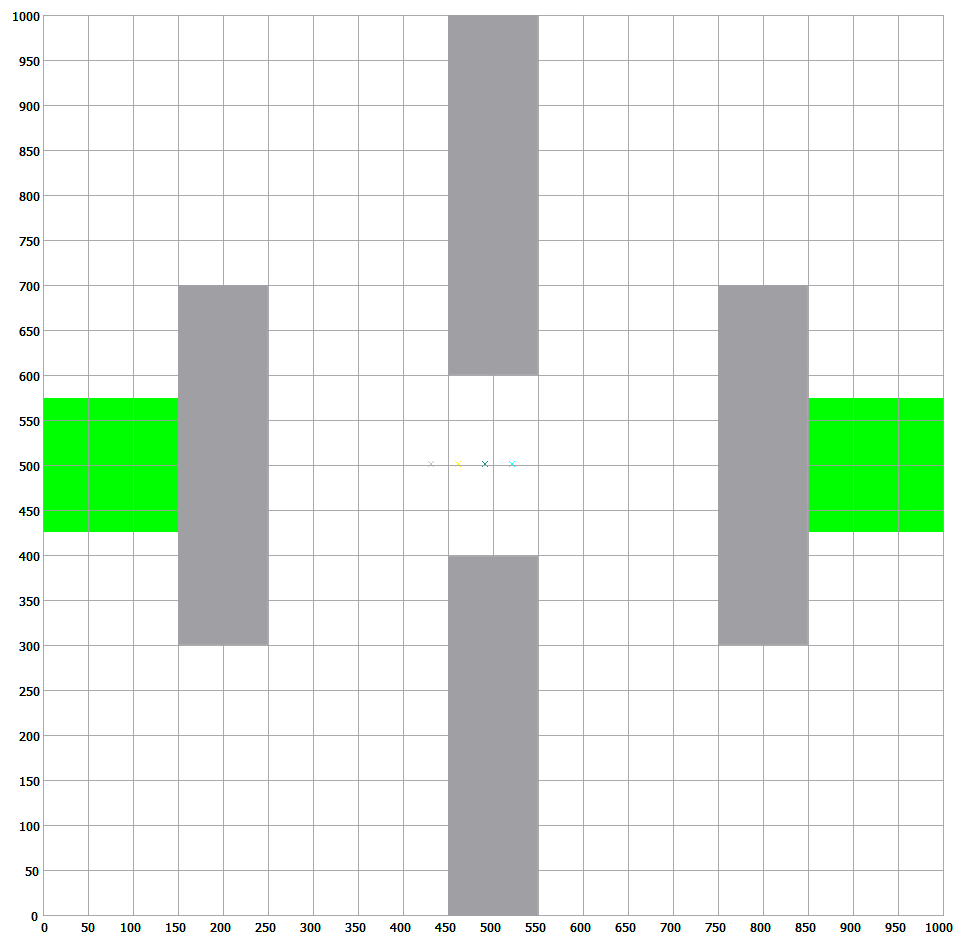
\includegraphics[scale=0.3]{obrazky/map1}

\caption{Map with goals unsuitable for grouping \label{fig:Map-with-goals}}
\end{figure}


\begin{figure}
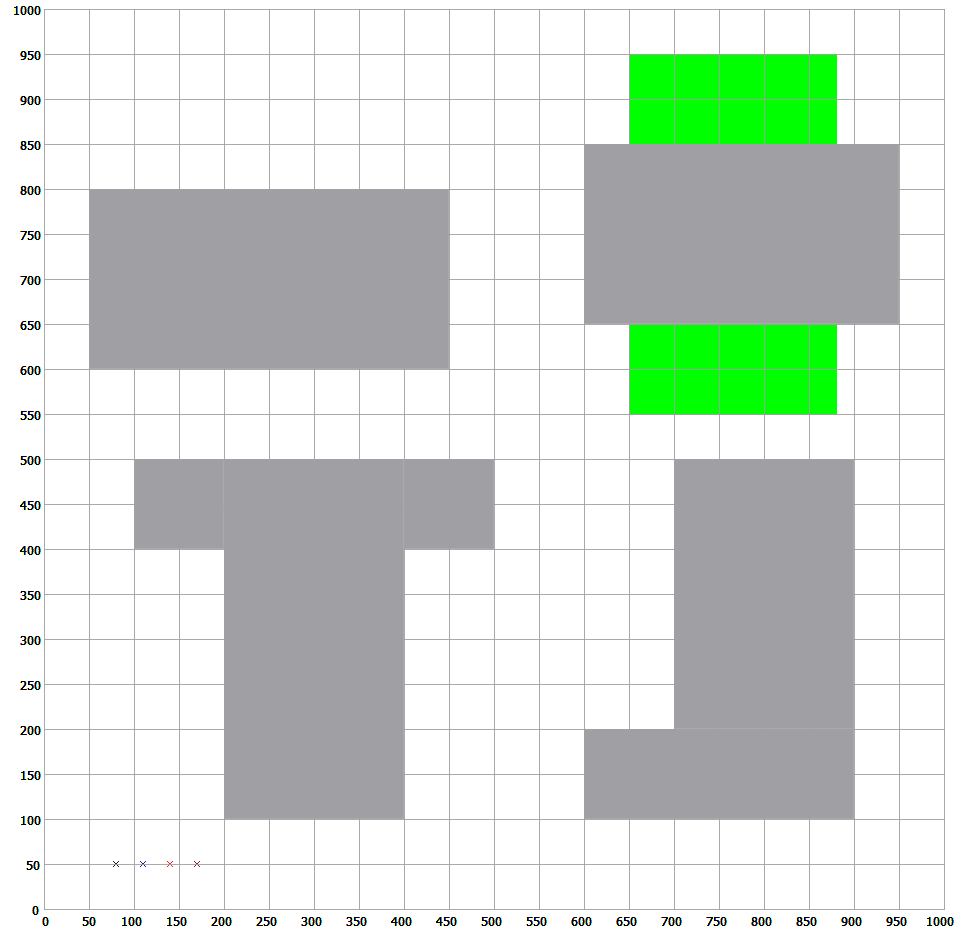
\includegraphics[scale=0.3]{obrazky/map2}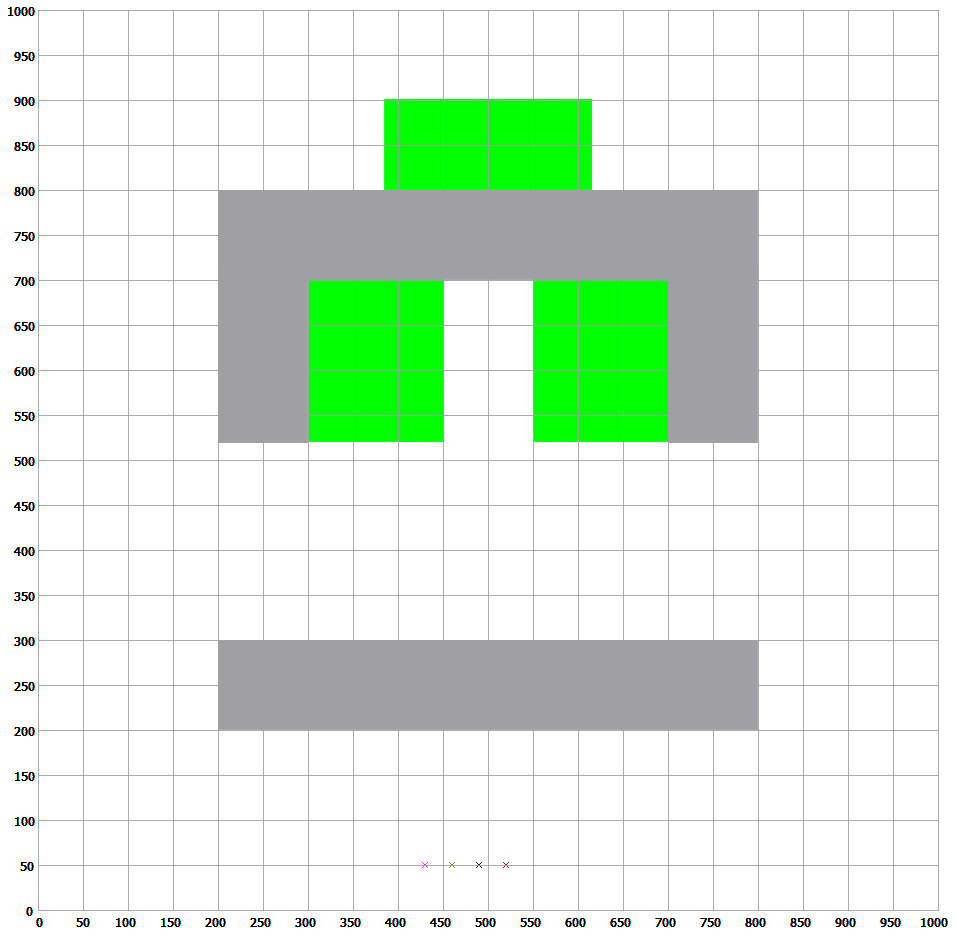
\includegraphics[scale=0.3]{obrazky/map5}

\caption{Maps with goals suitable for grouping \label{fig:Maps-with-goals}}
\end{figure}



\chapter[Paths straightening]{Paths straightening \label{chap:Paths-straightening}}

RRT-Path algorithm checks crossing paths between neighbouring states,
so between nth state and n+1-th \marginpar{todo: zjistit, jak je to správně anglicky}
state no trajectories are crossing each other. But between states
trajectories are still crossing. In this image \ref{fig:Crossing-paths}
is shown path found by RRT-Path. Every colour marks one state in RRT-Path.
As we can see, check in algorithm prevents from crossing path between
neighbouring states, but crossing of paths in different times can
not be easily prevented. We can see in image, that paths cross between
points J (yellow), M (light green) and H (orange), K (yellow), so
there is no easy approach to prevent path collisions between n-2-th
state and nth state. Optimization by Dubins curves shortens trajectory
of UAVs, so UAVs could be in these trajectories in different time,
so there could be collisions after optimization. Another complication
occurs, when time difference between two states is too low, then UAVs
could collide, because in reality UAV can not follow path precisely,
but only with some errors.

\begin{figure}
\caption{Crossing paths \label{fig:Crossing-paths}}


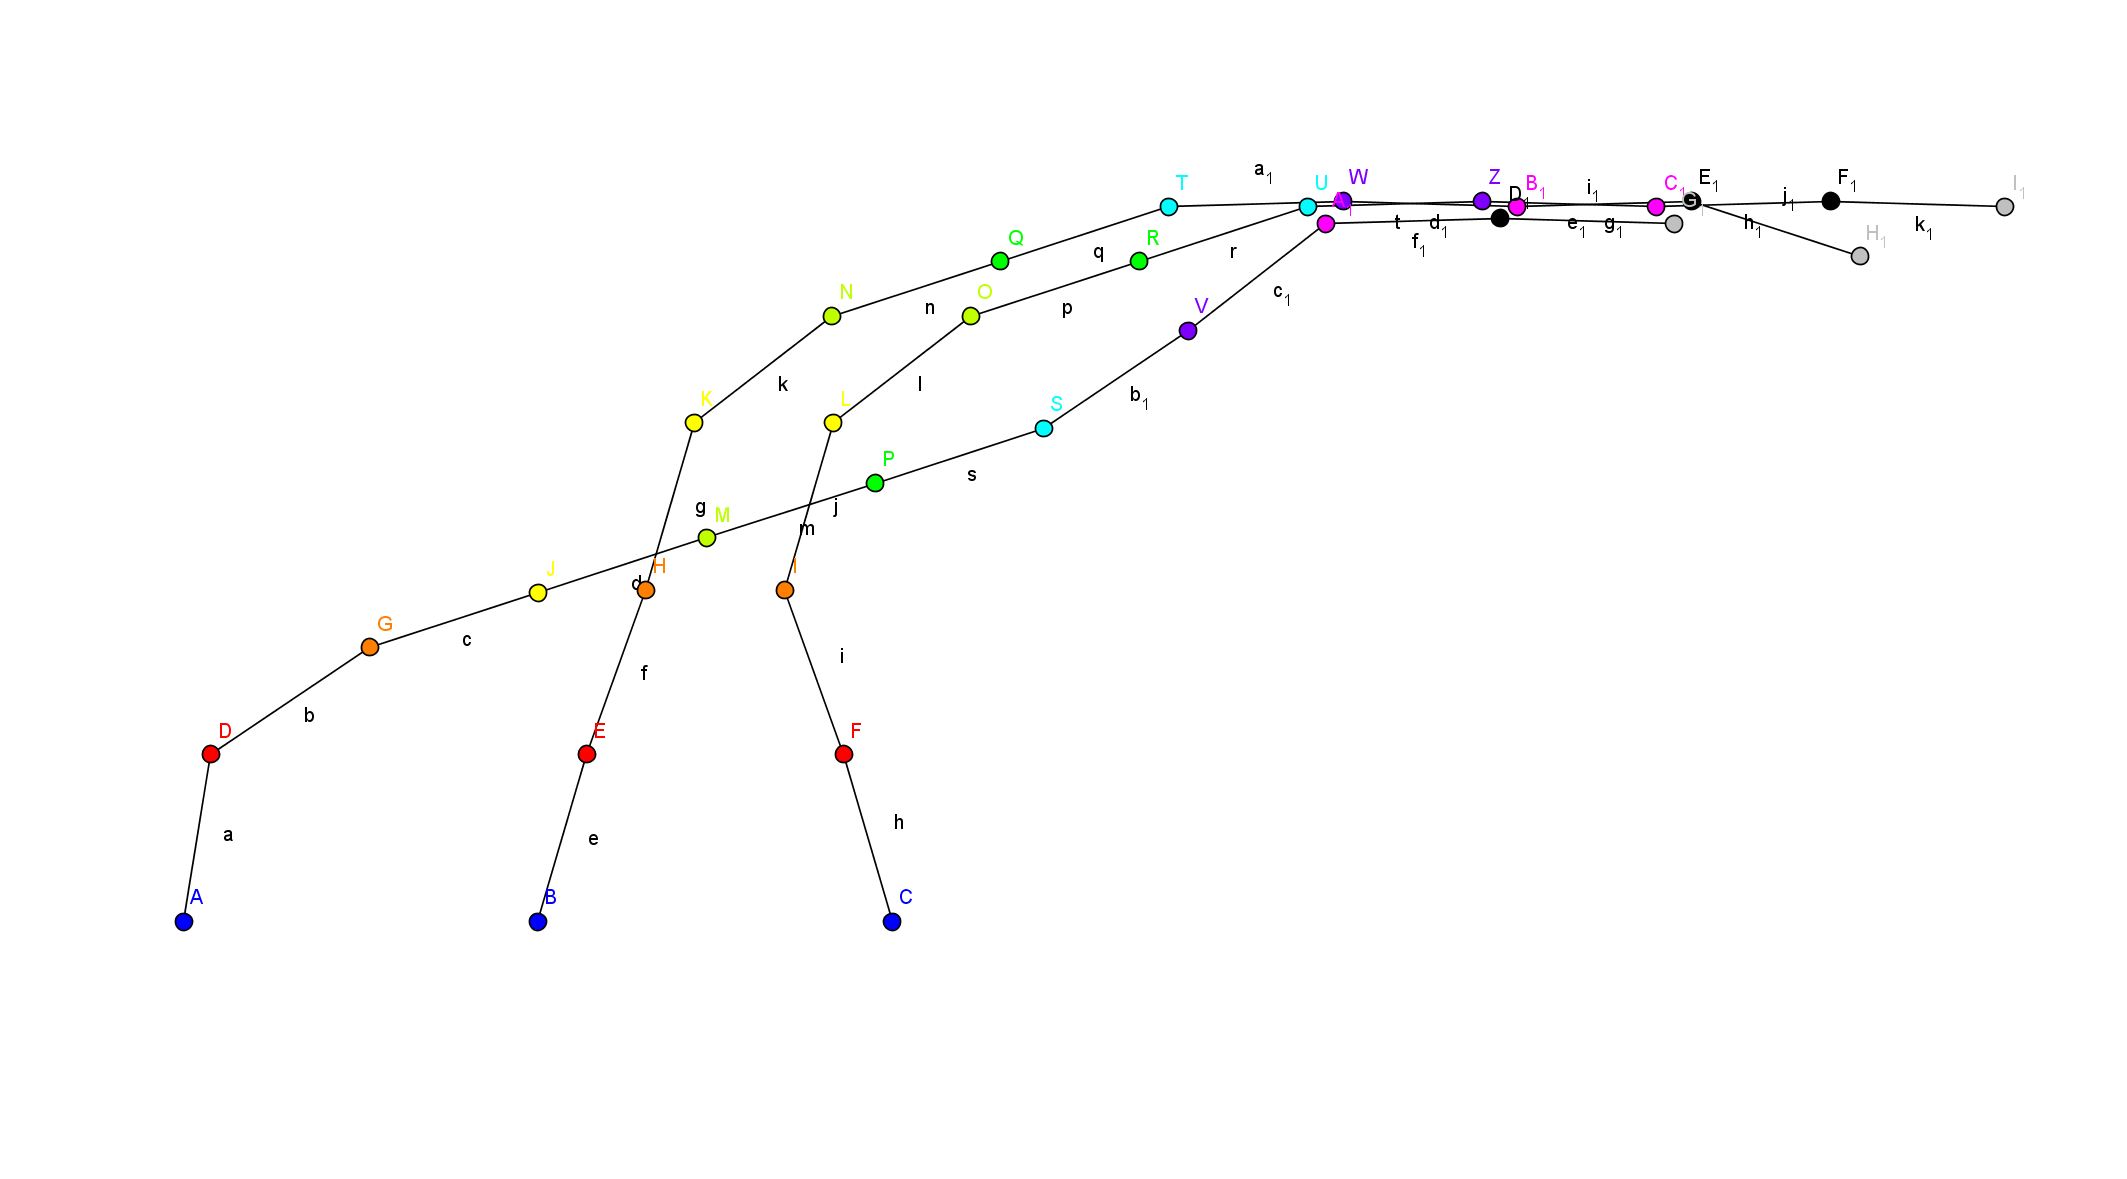
\includegraphics[scale=0.3]{obrazky/crossingPathReal1}
\end{figure}
I tried to straighten crossing trajectories, but all attempts failed.
Straightening was done by switching parts of crossing paths from the
earliest crossing state to end. But then paths had different lengths,
which was unsuitable for path planning for swarm. This can be done
by adding ``waiting'' points, points in different state but with
same position in different time. But then is really hard to straighten
longer path with many crossings (this path is really short, paths
in other maps are much longer and more complicated). For motion model
with inertia is also really hard to deal with waiting states, which
complicates following of straightened trajectories. Due to all complications
mentioned above, this part was removed from algorithm. But it is possible
to add it, when better approach will be found.


\chapter[Motion model]{Motion model}

The RRT-Path algorithm is universal and works without motion model,
which is fine for holonomic robot, but usage of motion model allows
us to find path more feasible for swarm of UAVs than without using
of holonomic robot. For this purpose, car like model was chosen. Differential
equations of motion model in 3D from \cite{MartinSaskaPreucil} are
\begin{equation}
\begin{array}{ccc}
\dot{x}\left(t\right) & = & v\left(t\right)\sin\varphi\left(t\right)\\
\dot{y}\left(t\right) & = & v\left(t\right)\cos\left(t\right)\\
\dot{z}\left(t\right) & = & w\left(t\right)\\
\dot{\varphi}\left(t\right) & = & K\left(t\right)v\left(t\right)
\end{array}
\end{equation}
where $x\left(t\right),y\left(t\right),z\left(t\right)$ are coordinates
of UAV, $\varphi\left(t\right)$ represents heading of UAV, $v\left(t\right)$
is forward velocity, $K\left(t\right)$ is curvature, $w\left(t\right)$
is ascent velocity. $\begin{bmatrix}K\left(t\right) & w\left(t\right) & v\left(t\right)\end{bmatrix}$
represent input vector of motion model. Differential equations are
useful for representation in equations, but not useful for computer
algorithm. For usage in algorithm are better difference equations
instead of differential equations. When inputs are held constant in
each time interval between two time steps, difference equations are
\begin{equation}
\begin{array}{ccc}
x\left(k+1\right) & = & \begin{cases}
if\,K\left(k+1\right)\neq0\\
x\left(k\right)+\frac{1}{K\left(k+1\right)}\left(\sin\left(\varphi\left(k\right)+K\left(k+1\right)v\left(k+1\right)\Delta t\left(k+1\right)\right)-\sin\left(\varphi\left(k\right)\right)\right)\\
if\,K\left(k+1\right)=0\\
x\left(k\right)+v\left(k+1\right)\cos\left(\varphi\left(k\right)\right)\Delta t\left(k+1\right)
\end{cases}\\
y\left(k+1\right) & = & \begin{cases}
if\,K\left(k+1\right)\neq0\\
y\left(k\right)-\frac{1}{K\left(k+1\right)}\left(\cos\left(\varphi\left(k\right)+K\left(k+1\right)v\left(k+1\right)\Delta t\left(k+1\right)\right)-\cos\left(\varphi\left(k\right)\right)\right)\\
if\,K\left(k+1\right)=0\\
y\left(k\right)+v\left(k+1\right)\sin\left(\varphi\left(k\right)\right)\Delta t\left(k+1\right)
\end{cases}\\
z\left(k+1\right) & = & z\left(k\right)+w\left(k+1\right)\Delta t\left(k+1\right)\\
\varphi\left(k+1\right) & = & \varphi\left(k\right)+K\left(k+1\right)v\left(k+1\right)\Delta t\left(k+1\right)
\end{array}
\end{equation}



\chapter[Dubins curves]{Dubins curves}

Dubins curves, also called Dubins manoeuvrers or Dubins path were
published by Lester Eli Dubins in 1957 \cite{Dubins1957}. Dubins
path is optimal path for car like motion model. Path is optimal, when
car moves at constant forward speed. The other important constraint
is the maximum steering angle $\phi_{max}$, which results in a minimum
turning radius$\rho_{min}$. As the car travels, consider the length
of the curve in ${\cal W}=\mathbb{R}^{2}$ traced out by a pencil
attached to the centre of the car. The task is to minimize the length
of this curve as the car travels between any $q_{I}$ and $q_{G}$.
Due to $\rho_{min}$, this can be considered as a bounded-curvature
shortest-path problem. If $\rho_{min}=0$, then there is no curvature
bound, and the shortest path follows a straight line in $\mathbb{R}^{2}$.
In terms of a cost function, the criterion to optimize is

\begin{equation}
\ensuremath{{\displaystyle L(\tilde{q},\tilde{u})=\int_{0}^{t_{F}}\sqrt{\dot{x}(t)^{2}+\dot{y}(t)^{2}}dt}}
\end{equation}
, where $t_{F}$ is the time at which $q_{G}$ is reached, and a configuration
is denoted as $q=(x,y,\theta)$, $\tilde{x}_{t}$ denotes the function
$\tilde{x}_{t}:[0,t]\rightarrow X$, which is called the state trajectory
(or state history). This is a continuous-time version of the state
history, which was defined previously for problems that have discrete
stages. Similarly, $\tilde{u}_{t}$ denotes the action trajectory
(or action history),. If $q_{G}$ is not reached, then it is assumed
that $L(\tilde{q},\tilde{u})=\infty$. \cite{LaValle2006}

When considering constraints of inputs (actions) for motion model,
the system can be simplified to

\begin{equation}
\begin{array}{ccc}
\dot{x} & = & \cos\theta\\
\dot{y} & = & \sin\theta\\
\dot{\theta} & = & u
\end{array}
\end{equation}


in which $u$ is chosen from the interval $U=\left\{ -\tan\phi_{max},0,\tan\phi_{max}\right\} $.
For simplicity, assume that $\tan\phi=1$. The following results also
hold for any $\phi_{max}\in(0,\pi/2)$. 

\begin{table}
\caption{The three motion primitives from which all optimal curves for the
Dubins car can be constructed. \label{tab:The-three-motion}}


\begin{tabular}{|c|c|}
\hline 
Symbol & Steering u\tabularnewline
\hline 
\hline 
L & -1\tabularnewline
\hline 
S & 0\tabularnewline
\hline 
R & 1\tabularnewline
\hline 
\end{tabular}
\end{table}


It was shown in \cite{Dubins1957} that between any two configurations,
the shortest path for the Dubins car can always be expressed as a
combination of no more than three motion primitives. Each motion primitive
applies a constant action over an interval of time. Furthermore, the
only actions that are needed to traverse the shortest paths are $u\in\{-1,0,1\}$.
The primitives and their associated symbols are shown in \ref{tab:The-three-motion}.
The $S$ primitive drives the car straight ahead. The $L$ and $R$
primitives turn as sharply as possible to the left and right, respectively.
Using these symbols, each possible kind of shortest path can be designated
as a sequence of three symbols that corresponds to the order in which
the primitives are applied. Let such a sequence be called a word .
There is no need to have two consecutive primitives of the same kind
because they can be merged into one. Under this observation, ten possible
words of length three are possible. Dubins showed that only these
six words are possibly optimal:

\begin{equation}
\ensuremath{{\displaystyle \{LRL,\;RLR,\;LSL,\;LSR,\;RSL,\;RSR\}.}}
\end{equation}


The shortest path between any two configurations can always be characterized
by one of these words. These are called the Dubins curves.


\chapter[Optimization using Dubins curves]{Optimization using Dubins curves}

The Dubins curves are used to optimize trajectory found with RRT-Path
algorithm.

Whole optimization works as follows.

Two random states are chosen, which means one path as part of whole
trajectory for each UAV will be optimized. Beginning and ending point
of selected path are used as input to Dubins curve algorithm. 

Dubins curve is then sampled with same frequency used in RRT-Path
algorithm and is tested for feasibility. When the new path is feasible
and shorter than original path, the original path is replaced. and
distances of the original and new trajectory part are compared. When
new trajectory part is shorter, it is used instead of original trajectory
part.

This is repeated in cycle which stops when path is not shortened after
many (eg. 150) iterations or optimization is too slow and path is
shortened only by small distances (eg. shortening by 5\% per 1000
iterations). 


\chapter[Path re-sampling]{Path re-sampling\label{chap:Path-resampling}}

Motion model in RRT-Path algorithm uses constant input in range from
0.5 to 1 second. Smaller interval for constant input causes RRT-Path
algorithm to run for too long. When using too short constant input
interval, the tree has too many nodes, grows slowly and runs out of
memory much faster than longer interval. Interval longer than 1 second
makes UAVs unable to manoeuvre between smaller obstacles. Thus range
from 0.5 to 1 second was experimentally chosen as best interval. Using
$x$ seconds long constant input interval also means $\frac{1}{x}Hz$
frequency of points in resulting trajectory in output of the algorithm.
So the range from 0.5 to 1 second implies resulting frequency is in
range $1Hz$ to $2Hz$. 

Real UAVs in Multi-Robot Systems group at CTU use frequency 70Hz and
trajectories with lower frequency are linear interpolated to have
frequency 70Hz. That means frequency 2Hz is too low for real usage
because trajectory generated with this frequency would not be smooth
enough. 

Change of frequency before the RRT-Path algorithm makes the algorithm
unable to run efficiently in bigger maps, so this does not solve the
problem.

Another solution is to re-sample the path after Dubins curves. But
this method failed because after Dubins optimization, the curves had
different length and different constant input durations. 

The best solution for this problem is re-sampling of trajectory generated
by RRT-Path algorithm before it is optimized by Dubins curves. This
solution also has big advantage in Dubins curves optimization because
it results to shorter final path as will be shown in following experiment.


\section{Influence of re-sampling on Dubins curves optimization}

To demonstrate the optimization, I created map and let the RRT-Path
algorithm find the trajectories for UAVs. The map with trajectories
can be seen in \ref{fig:Path-before-Dubins}. Obstacles are grey rectangles,
AoI is green rectangle and each UAV has trajectory marked with different
colour. For measuring of influence of re-sampling of path to Dubins
curves optimization, I picked frequencies: 1 Hz (initial frequency
used in RRT-Path algorithm), 2 Hz, 4 Hz, 6 Hz, 8 Hz, 10 Hz, 12 Hz,
14 Hz, 16 Hz, 18 Hz, 20 Hz.

\begin{figure}
\caption{Path before Dubins curves optimization\label{fig:Path-before-Dubins}}
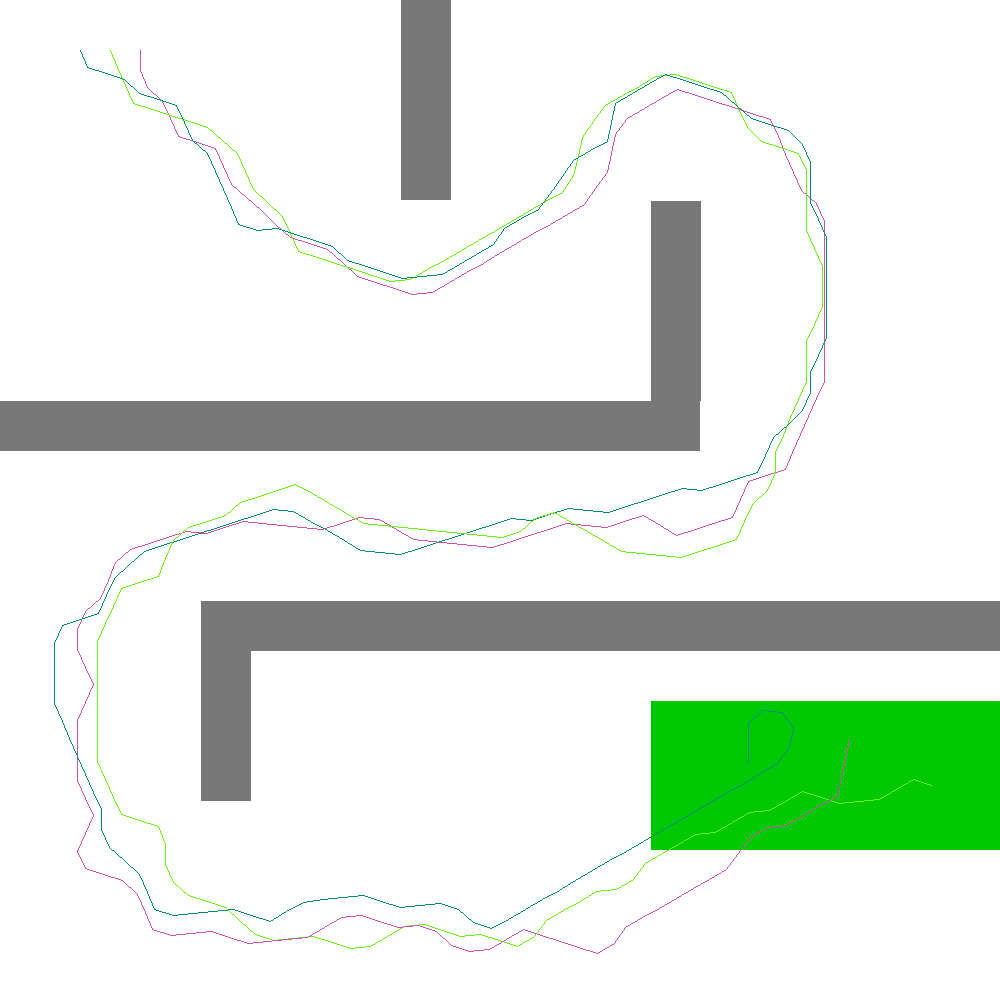
\includegraphics[scale=0.3]{obrazky/pathBeforeDubins}
\end{figure}


As stated above, due to time and memory consumption, each optimization
is stopped after 150 iterations where optimization did not shorten
the path or when speed of path shortening was slower than 5\% of original
path length per 1000 iterations.

For each frequency, the optimization process was run 100 times to
obtain relevant results because of using random numbers during the
optimization.

Following table shows average total, minimal and maximal distance
of all trajectories from 100 optimizations after the re-sampling and
optimization.

\begin{table}
\caption{Re-sampling and optimization results\label{tab:Re-sampling-and-optimization}}


\begin{tabular}{|c|c|c|c|}
\hline 
Frequency {[}Hz{]} & Minimal distance {[}m{]} & Maximal distance {[}m{]} & Average distance {[}m{]}\tabularnewline
\hline 
\hline 
1 & 8582.18 & 8849.7 & 8721.2904\tabularnewline
\hline 
2 & 8311.65 & 8548.81 & 8430.23\tabularnewline
\hline 
4 & 8366.88 & 8393.09 & 8379.985\tabularnewline
\hline 
6 & 8248.9 & 8275.7 & 8262.3\tabularnewline
\hline 
8 & 8249.88 & 8378.51 & 8314.195\tabularnewline
\hline 
10 & 8286.22 & 8472.2 & 8379.21\tabularnewline
\hline 
12 & 8302.51 & 8309.2 & 8307.6613\tabularnewline
\hline 
14 & 8303.18 & 8303.18 & 8303.18\tabularnewline
\hline 
16 & 8363.92 & 8363.92 & 8363.92\tabularnewline
\hline 
18 & 8510.32 & 8510.32 & 8510.32\tabularnewline
\hline 
20 & 8194.22 & 8194.22 & 8194.22\tabularnewline
\hline 
\end{tabular}
\end{table}


The results are also shown in graph \ref{fig:Re-sampling-and-optimization}.
On the graph we can see that initial frequency 1 Hz has worst results
and the frequency 20 Hz has best results. We can also see that in
frequency 14 Hz and higher, all 100 iterations had same results, the
minimum, maximum and mean value are the same. But the second best
frequency in terms of minimal, maximal and mean value is 6 Hz and
even the worst optimization in 6 Hz has smaller total distance than
8 to 18 Hz. 

\begin{figure}


\caption{Re-sampling and optimization results graph \label{fig:Re-sampling-and-optimization}}


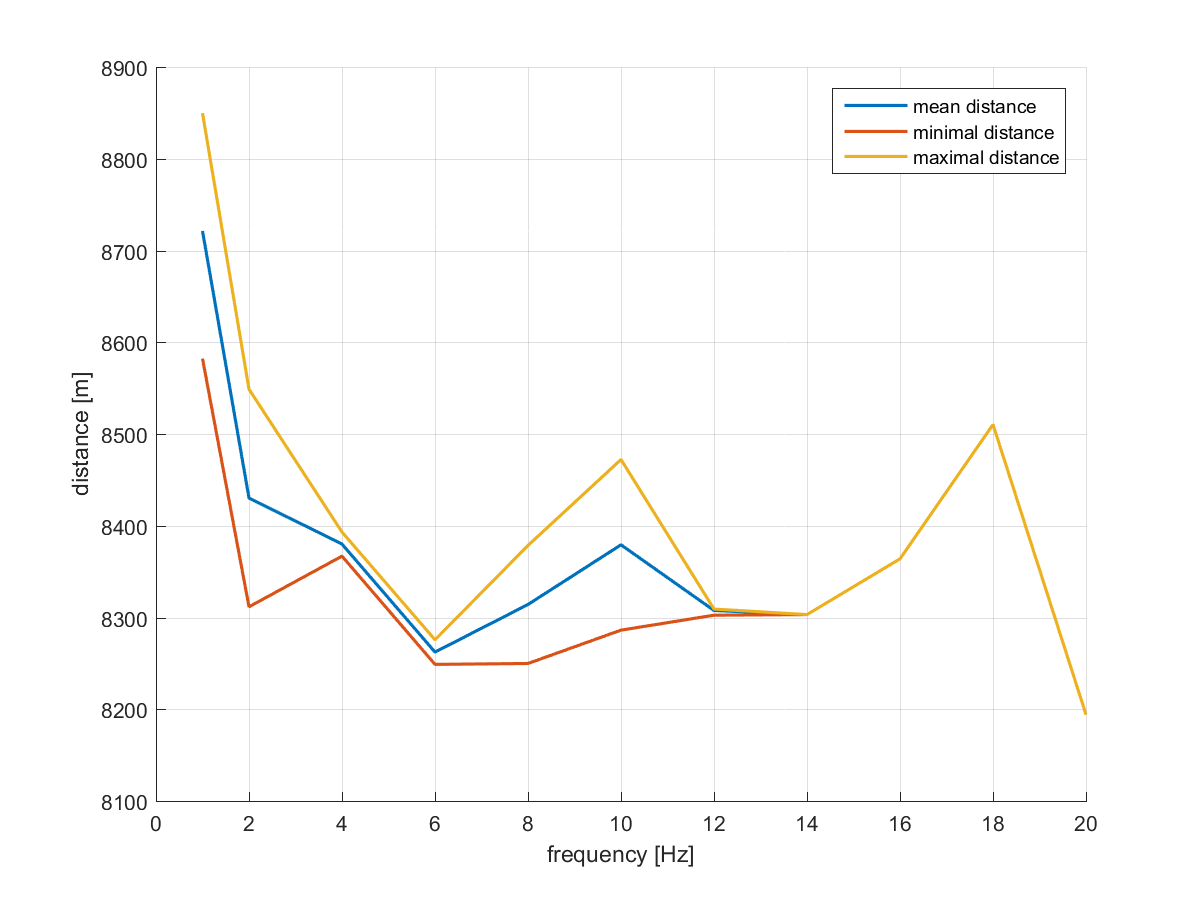
\includegraphics[scale=0.7]{obrazky/frequencyDependence}
\end{figure}


Depending on re-sampling frequency, the courses of optimization are
also different.

Here we can see mean values and standard deviations for different
frequencies, divided to two graphs for better lucidity. 

\begin{figure}


\caption{Time course of optimization}
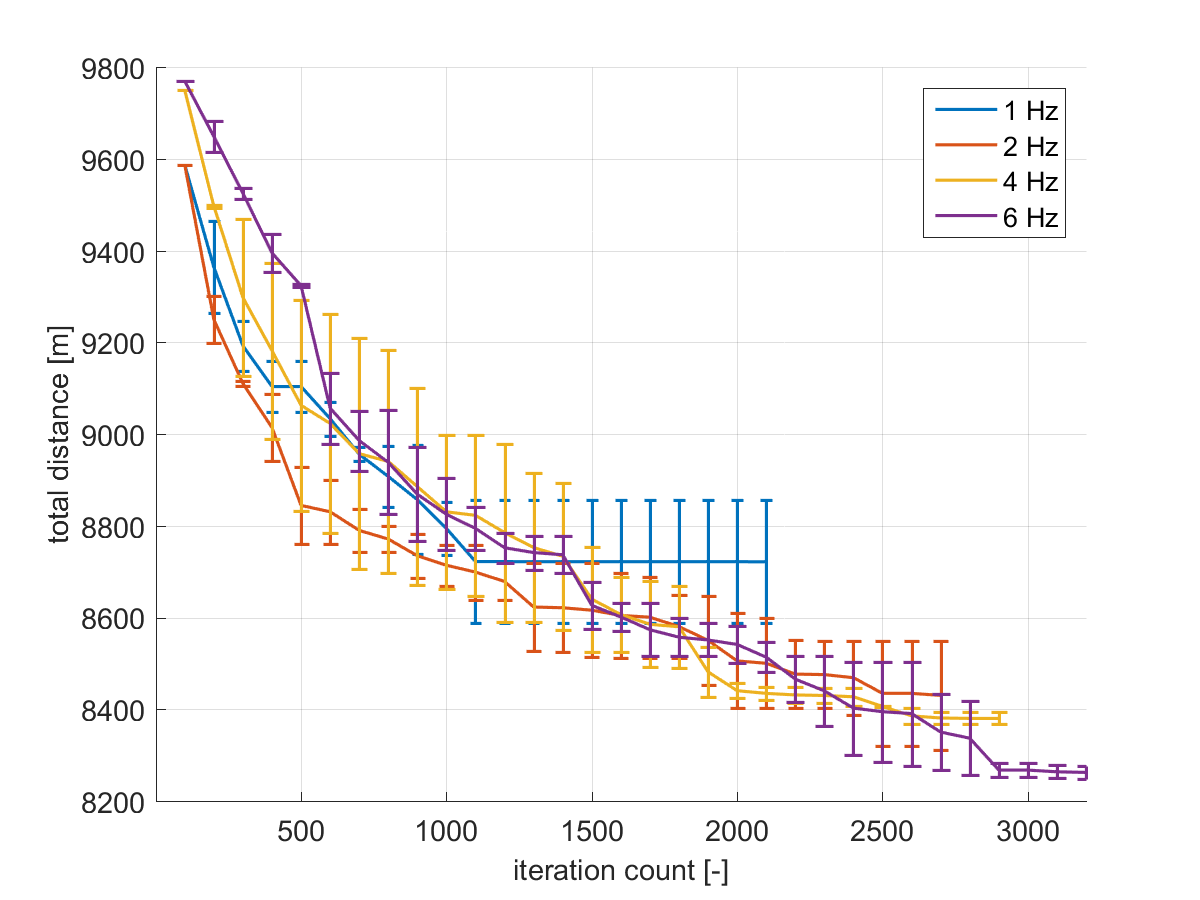
\includegraphics[scale=0.7]{obrazky/lowFrequenciesErrors}

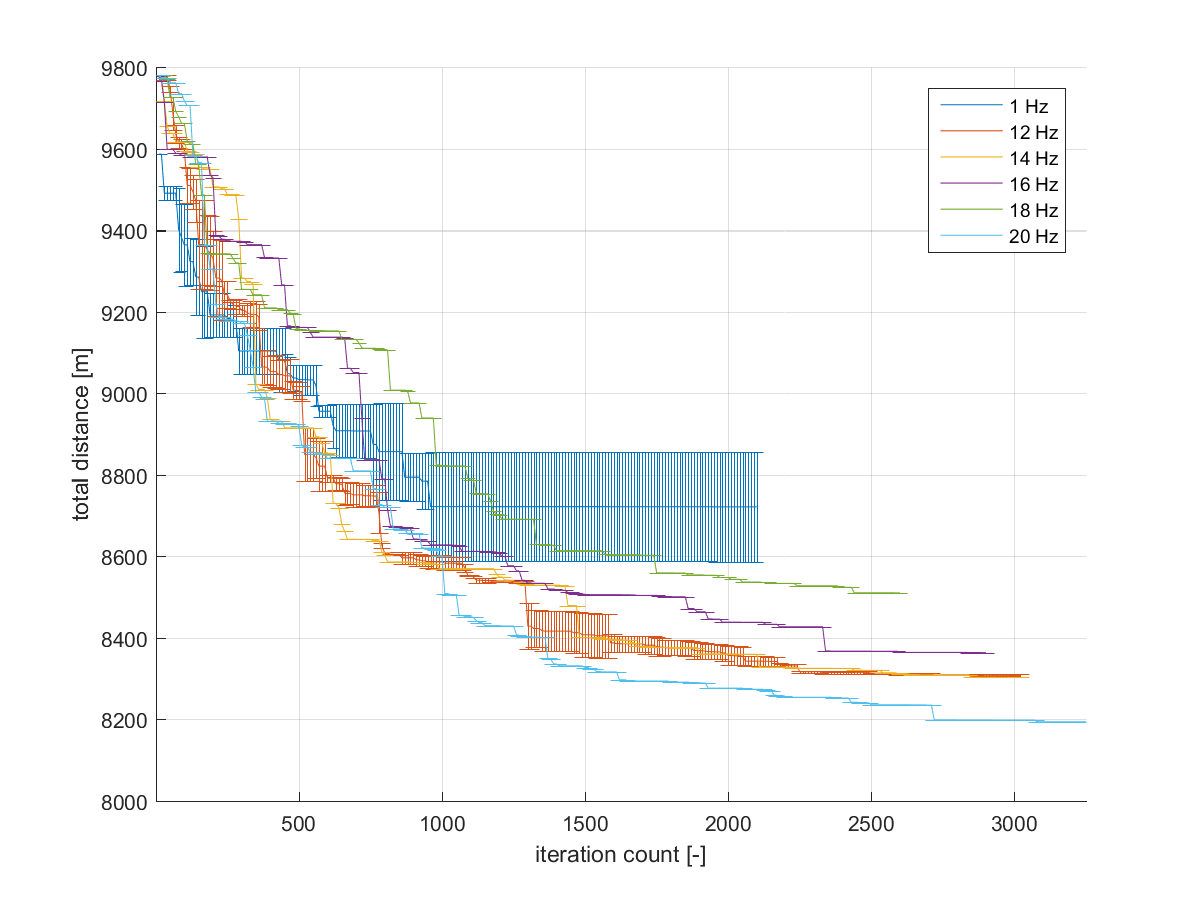
\includegraphics[scale=0.7]{obrazky/highFrequenciesErrors}

\end{figure}



\chapter[Implementation]{Implementation}

This part will cover implementation of algorithm, which was used for
simulations. Whole codebase can be found at \href{https://github.com/racinmat/AutonomousSurveillanceBachelorThesis}{this github repository}.


\section{External libraries}

In implementation are used some external libraries. Every used library
is mentioned here.\href{http://www.boost.org/}{Boost libraries} is
used for smart pointers, libraries for Dubins curves are from Master
Thesis by Petr Váňa\cite{Vana2015}. Generating of JSON from C++ object
is done via \href{http://www.codeproject.com/Articles/20027/JSON-Spirit-A-C-JSON-Parser-Generator-Implemented}{Json Spirit}
library. Another external library is \href{http://gamma.cs.unc.edu/V-COLLIDE/}{V-Collide}
from The University of North Carolina at Chapel Hill. 

Because V-Collide sources were written in 1997 and because I used
C++11 compiler to compile my source codes, I had to rewrite part of
this library for compatibility and to make public API easier to use.
Modifications can be seen in \href{https://github.com/racinmat/VCollide2}{this github repository}. 

Last use external library is QT, which was used to create platform
independent GUI.


\section{Code structure and services}

Here is shown brief UML scheme demonstrating dependency diagram of
codebase. To keep diagram simple, only services are displayed, other
classes, which are not services, were left out for lucidity. Diagram
was generated using software \href{http://staruml.io/}{StarUML}

\begin{figure}
\caption{Dependency diagram \label{fig:Dependency-diagram}}


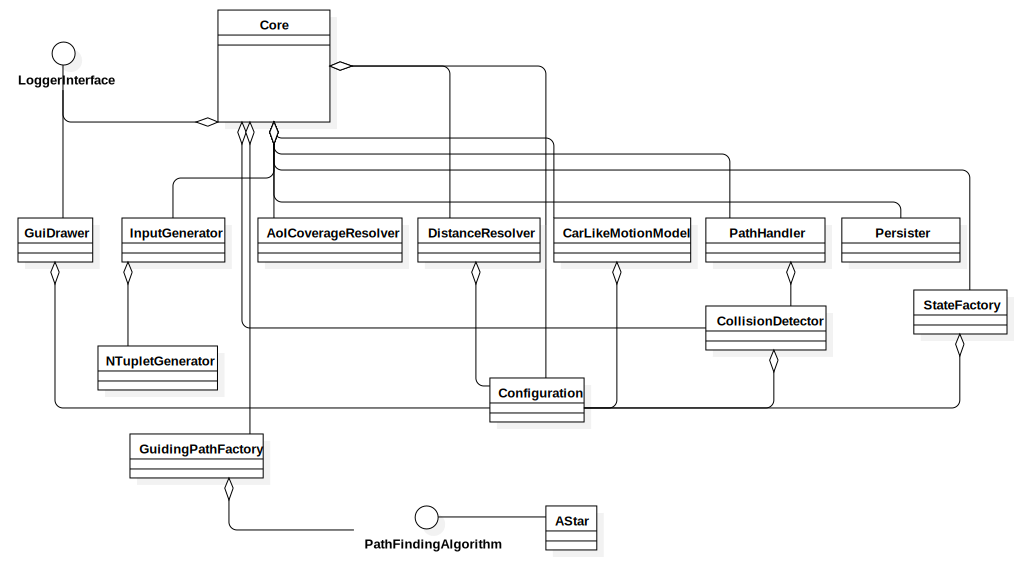
\includegraphics[scale=0.4]{obrazky/umlSchema}
\end{figure}


Core class holds core of whole Application and has all other classes
as dependencies, as is shown in image \ref{fig:Dependency-diagram}. 

As mentioned in \ref{chap:Algorithm} chapter Configuration is DTO
for all configuration variables, but to keep reasonable amount of
classes, Configuration is also service, which delegates all configuration
changes from GUI to Core class. Configuration and GuiDrawer implementation
LoggerInterface are the only connections between Core and GUI.

State factory creates State classes according to Factory pattern.
State class represents state in RRT-Path algorithm. State has coordinates
and rotations for all UAVs.

Persister persists found path to JSON using Json Spirit library.

PathHandler serves as utils class for manipulations with path (vector
of State classes).

CarLikeMotionModel holds motion model algorithm.

InputGenerator is used to generate inputs to motion model.

NTupletGenerator only generates variation with repeating for given
input.

DistanceResolver counts distances between two states and distance
of path.

AoICoverageResolver determines cost function for states,where all
UAVs are in AoIs.

GuidingPathFactory is wrapper for PathFindingAlgorithm interface and
is used by Core to find guiding path. 

Implementation of PathFindingAlgorithm is AStart class.

\bibliographystyle{plainnat}
\phantomsection\addcontentsline{toc}{chapter}{\bibname}\bibliography{bibliography}


\cleardoublepage{}
\end{document}
